\documentclass[tikz,border=3mm]{standalone}
\usepackage{tikz}
\usetikzlibrary{angles,quotes,calc,intersections}
\begin{document}
% TikZ 1
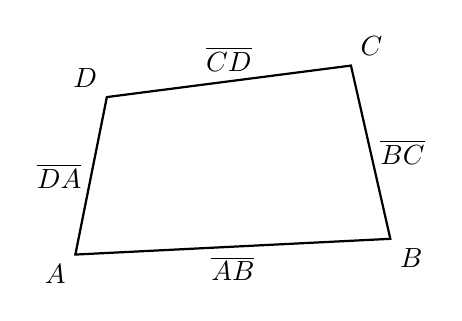
\begin{tikzpicture}[scale=1]
\coordinate (A) at (0,0); \coordinate (B) at (4,0.2); \coordinate (C) at (3.5,2.4); \coordinate (D) at (.4,2);
\draw[thick] (A)--(B)--(C)--(D)--cycle;
\foreach \p/\pos in {A/below left,B/below right,C/above right,D/above left}{\node[\pos] at (\p) {$\p$};}
\node[below] at ($(A)!0.5!(B)$) {$\overline{AB}$};
\node[right] at ($(B)!0.5!(C)$) {$\overline{BC}$};
\node[above] at ($(C)!0.5!(D)$) {$\overline{CD}$};
\node[left] at ($(D)!0.5!(A)$) {$\overline{DA}$};
\end{tikzpicture}
\hspace{1cm}
% TikZ 2
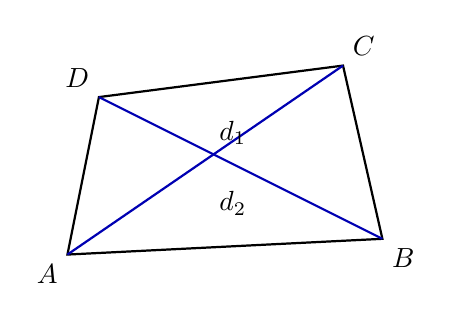
\begin{tikzpicture}[scale=1]
\coordinate (A) at (0,0); \coordinate (B) at (4,0.2); \coordinate (C) at (3.5,2.4); \coordinate (D) at (.4,2);
\draw[thick] (A)--(B)--(C)--(D)--cycle;
\draw[blue!70!black,thick] (A)--(C);
\draw[blue!70!black,thick] (B)--(D);
\foreach \p/\pos in {A/below left,B/below right,C/above right,D/above left}{\node[\pos] at (\p) {$\p$};}
\node at (2.1,1.55) {$d_1$};
\node at (2.1,.65) {$d_2$};
\end{tikzpicture}

\vspace{1cm}

% TikZ 3
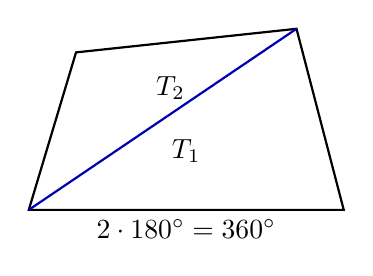
\begin{tikzpicture}[scale=1]
\coordinate (A) at (0,0); \coordinate (B) at (4,0); \coordinate (C) at (3.4,2.3); \coordinate (D) at (.6,2);
\draw[thick] (A)--(B)--(C)--(D)--cycle;
\draw[blue!70!black,thick] (A)--(C);
\node at (2,.75) {$T_1$};
\node at (1.8,1.55) {$T_2$};
\node[below] at (2,0) {$2\cdot180^{\circ}=360^{\circ}$};
\end{tikzpicture}
\hspace{1cm}
% TikZ 4
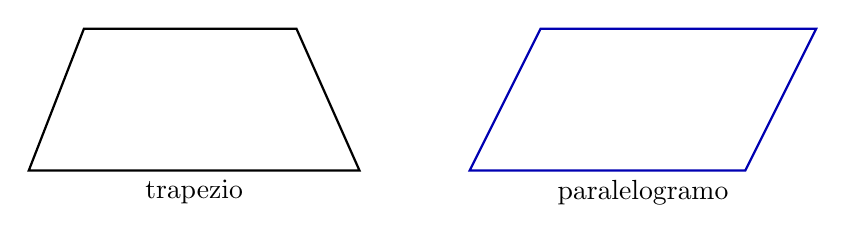
\begin{tikzpicture}[scale=1]
\coordinate (A) at (0,0); \coordinate (B) at (4.2,0); \coordinate (C) at (3.4,1.8); \coordinate (D) at (.7,1.8);
\draw[thick] (A)--(B)--(C)--(D)--cycle;
\node[below] at (2.1,0) {trapezio};
\coordinate (E) at (5.6,0); \coordinate (F) at (9.1,0); \coordinate (G) at (10,1.8); \coordinate (H) at (6.5,1.8);
\draw[thick,blue!70!black] (E)--(F)--(G)--(H)--cycle;
\node[below] at (7.8,0) {paralelogramo};
\end{tikzpicture}

\vspace{1cm}

% TikZ 5
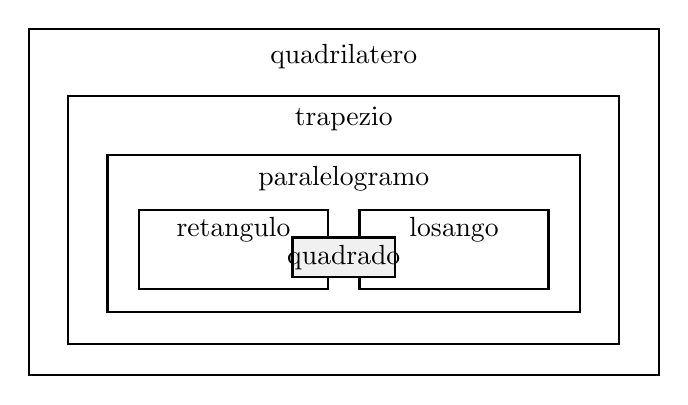
\begin{tikzpicture}[scale=1]
\draw[thick] (0,0) rectangle (8,4.4);
\node at (4,4.05) {quadrilatero};
\draw[thick] (.5,.4) rectangle (7.5,3.55);
\node at (4,3.25) {trapezio};
\draw[thick] (1,0.8) rectangle (7,2.8);
\node at (4,2.5) {paralelogramo};
\draw[thick] (1.4,1.1) rectangle (3.8,2.1);
\node at (2.6,1.85) {retangulo};
\draw[thick] (4.2,1.1) rectangle (6.6,2.1);
\node at (5.4,1.85) {losango};
\draw[thick,fill=gray!12] (3.35,1.25) rectangle (4.65,1.75);
\node at (4,1.5) {quadrado};
\end{tikzpicture}
\end{document}
